\documentclass[12pt]{article}
\usepackage[english]{babel}
\usepackage{graphicx, amsmath, mathtools, listings, color, caption, rotating, subfigure, fullpage, textcomp, enumerate, float, amssymb}

\newcommand{\iid}{\stackrel{\mathrm{iid}}{\sim}}

\lstset{
	language=R,
	keywordstyle=\bfseries\ttfamily\color[rgb]{0,0,1},
	identifierstyle=\ttfamily,
	commentstyle=\color[rgb]{0.133,0.545,0.133},
	stringstyle=\ttfamily\color[rgb]{0.627,0.126,0.941},
	showstringspaces=false,
	basicstyle=\tiny,
	numberstyle=\scriptsize,
	numbers=left,
	stepnumber=1,
	numbersep=10pt,
	tabsize=2,
	breaklines=true,
	breakatwhitespace=false,
	aboveskip={1.5\baselineskip},
  columns=fixed,
  upquote=true,
  extendedchars=true,
}

\begin{document}
\begin{center}
Homework 1 Possible Solutions
\end{center}

\section*{Problem 1}
\begin{enumerate}[(a)]
\item \begin{align*}
	R_{tr} ( \hat(\beta ) ) &= \frac{1}{N} \sum_{i=1}^n \left( y_i - \beta^T x_i \right)^2 
			< \frac{1}{N-p} \sum_{i=1}^n \left( y_i - \beta^T x_i \right)^2 = \text{MSE} \\
			& \Rightarrow E(R_{tr}) < E(MSE) = \sigma^2
	\end{align*}
	
\item \begin{align*}
	E ( R_{te}( \hat(\beta ) ) &= 
	\frac{1}{M} E \sum_{i=1}^M \left( \tilde{y_i} - \hat{\beta}^T \tilde{x_i} \right)^2 \\
%
	&= \frac{1}{M} E \left[ \sum_{i=1}^M \left(  \left( \tilde{y_i} - \hat{\beta}^T \tilde{x_i} \right) + \left( \beta^T \tilde{x_i} - \beta^T \tilde{x_i} \right) \right)^2 \right] \\
%	
	&= \frac{1}{M} E \left[ \sum_{i=1}^M \left( \tilde{y_i} - \beta^T \tilde{x_i} \right)^2 + \sum_{i=1}^M \left( \hat{\beta^T} \tilde{x_i} - \beta^T \tilde{x_i} \right)^2 \right] \\
%
	&= \frac{1}{M} E \sum_{i=1}^M \left( \tilde{y_i} - \beta^T \tilde{x_i} \right)^2 +
	\frac{1}{M} E \sum_{i=1}^M \left( \hat{\beta^T} \tilde{x_i} - \beta^T \tilde{x_i} \right)^2 \\
%
	&= \sigma^2 + \text{(something squared)} > \sigma^2
\end{align*}
\item On average, the training set error will be \emph{less} than the testing set error. This has many implications in both prediction and inference.

\item The attached code generates random noise data sets, calculates training and test set risks, then makes a histogram based on 100 simulations. The blue line is $\sigma^2 = 1$, and the red line is the average risk for training and test set.
\begin{lstlisting}
generateData = function(n, m, p){
  #Takes in training and testing sample sizes and number of predictors.
  #Generates simple noise data
  yTrain = rnorm(n) #Responses
  xTrain = matrix(rnorm(n*p), ncol=p) #Predictors
  
  yTest = rnorm(m) #Responses
  xTest = matrix(rnorm(m*p), ncol=p) #Predictors
  list(yTrain=yTrain, xTrain=xTrain, yTest=yTest, xTest=xTest)
}

calcRisks = function(trainTest){
  # Takes in training and testing data in a list.
  #Unrolls into matrices, then calculates
  # the training and testing errors (scalars). Returns a 2-vector.
  yTrain = trainTest$yTrain
  xTrain = trainTest$xTrain
  yTest = trainTest$yTest
  xTest = trainTest$xTest

  #Compute training OLS estimate, get residuals/coeffs from it.
  trainLM = lm(yTrain ~ xTrain)
  trainResid = trainLM$resid
  trainCoeffs = trainLM$coefficients

  #Use training OLS estimates to make testing fits. Compute errors.
  testFits = cbind(rep(1,nrow(xTest)), xTest) %*% trainCoeffs
  testResid = yTest - testFits
  
  riskTrain = 1/length(yTrain) * sum(trainResid^2)
  riskTest = 1/length(yTest) * sum(testResid^2)
  c(riskTrain, riskTest)
}

n = 100 #Train sample size
m = 100 #Test sample size
p = 10 #Number of predictors
nsim = 100 #Number of simulations

simErrors = t(sapply(1:nsim, function(i) calcRisks(generateData(n, m, p))))
par(mfrow=1:2)
hist(simErrors[,1], main='Histogram of Training Risk', xlab='Training Risk')
abline(v = mean(simErrors[,1]), col='red', lwd=4)
abline(v = 1, col='blue', lwd=4)
hist(simErrors[,2], main='Histogram of Testing Risk', xlab='Testing Risk')
abline(v = mean(simErrors[,2]), col='red', lwd=4)
abline(v = 1, col='blue', lwd=4)
\end{lstlisting}
\begin{figure}[H] \center
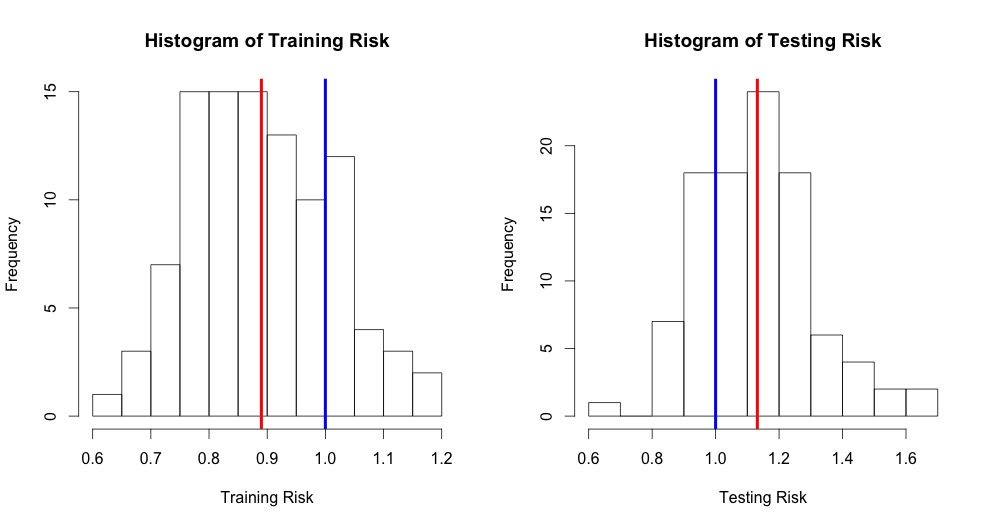
\includegraphics[scale=.4]{RiskHist.jpeg}
\end{figure}
\end{enumerate}

\section*{Problem 2}
\begin{enumerate}[(a)]
\item We want a confidence interval for $\sum_{j=0}^3 \beta_j x_0^j$. This is accomplished by noting that (at least asymptotically) the OLS estimates are normal, so a linear combination is normal as well. We do not know $\sigma^2$ however, and estimating it, we incur a small penalty. Because we must estimate $\sigma^2$, the linear combination, when suitably standardized, will have a $t_{n-p}$ distribution instead of a normal. The point estimate will be $\hat{f}(x_0) =  x_0 \hat{\beta}$, $\beta \in \mathbb{R}^4$, and where, forgive the abuse of notation, $x_0 = (1, x_0, x_0^2, x_0^3)$. The variance is
$$ \text{V}(\hat{f}(x_0)) = x_0' \text{V}( \hat{\beta}) ) x_0 = \sigma^2 \cdot x_0' \cdot (X'X)^{-1} \cdot x_0. $$
Not knowing $\sigma^2$, we use the plug-in estimator, MSE, and argue $\left[ \text{V}(\hat{f}(x_0))\right]^{-1/2} \hat{f}(x_0)$ is t-distributed with $n-p$ degrees of freedom. A confidence interval for $f(x_0)$ is 
$$\hat{f}(x_0) \pm \sqrt{\text{MSE} \cdot x_0' \cdot (X'X)^{-1} \cdot x_0} \cdot t_{n-p, 1-\alpha/2}.$$
\item The confidence set method follows by applying the Scheff\'{e} Method, which creates simultaneous intervals for $\beta$, then using this interval to come up with all possible linear combinations for $\sum_{i=0}^3 \beta_j x_0^j$, $\forall x_0$. This interval is 
$$\hat{f}(x_0) \pm \sqrt{\text{MSE} \cdot x_0' \cdot (X'X)^{-1} \cdot x_0 \cdot \chi_{4, 1-\alpha}^2}.$$
There was some note about using $p F_{p, n-p, 1-\alpha}$. The $\chi^2$ method is asymptotic. These methods are equivalent for large $n$ and small $p/n$, though the $F$ method is based on non-asymptotic normality where we need to estimate $\sigma^2$, and the $\chi^2$ relies on Central Limit Theorem.

The method in (a) needs only give coverage to the point $\hat{f}(x_0)$, whereas the method in (b) gives proper coverage for any linear combination of the form $\sum_{j=0}^3 \beta_j x_0^j$ we choose. This means we have to be a bit more conservative than if we could make statements about a particular $x_0$.
\begin{lstlisting}
income = read.csv("http://www-bcf.usc.edu/~gareth/ISL/Income1.csv")[,-1]
incomeModel = lm(Income ~ Education + I(Education^2) + I(Education^3), data=income)
pointwiseCI = predict(incomeModel, interval = "confidence")

multiplier = sqrt(qchisq(.95, 4))
familywiseCI = predict(incomeModel, se.fit=TRUE)
scheffeInterval = data.frame(fit = familywiseCI$fit,
                             lwr = familywiseCI$fit - multiplier * familywiseCI$se.fit,
                             upr = familywiseCI$fit + multiplier * familywiseCI$se.fit)

plot(Income ~ Education, data=income)
legend("topleft", c("Fitted Values", "Pointwise CI", "Familywise CI"), 
       lty = c(1, 2, 4), col = c("red", "blue", "purple")) #Add a legend
#Plot Pointwise CI
lines(income$Education, pointwiseCI[,1], col = "red")
lines(income$Education, pointwiseCI[,2], lty = 2, col = "blue")
lines(income$Education, pointwiseCI[,3], lty = 2, col = "blue")
#Plot Scheffe
lines(income$Education, scheffeInterval[,2], lty = 4, col = "purple")
lines(income$Education, scheffeInterval[,3], lty = 4, col = "purple")
\end{lstlisting}
\begin{figure}[H] \center
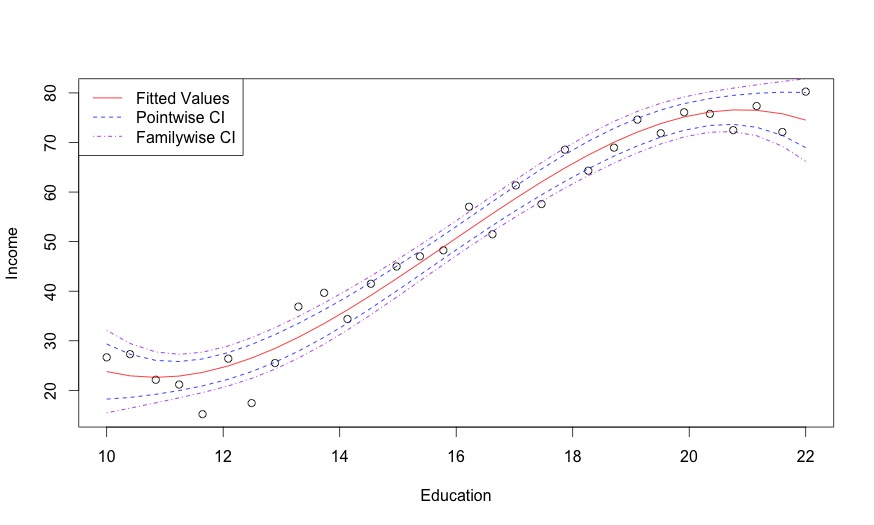
\includegraphics[scale=.6]{Pr2b.jpeg}
\end{figure}


\end{enumerate}



\section*{Problem 3}
\begin{enumerate}[(a)]
\item A possible rule would be to classify observations to $Y=1$ if $P(Y=1) = \text{sigmoid}(\hat{\beta}^T X) \geq 0.5$. This is equivalent to classifying to $Y=1$ if $\hat{\beta}^T X \geq 0$. 
\begin{lstlisting}
load("hw1prob3.Rdata")
logisticY1 = glm(y1~x, family='binomial')
plot(x[,1], x[,2], col=c("red","blue")[y1+1], pch = c('o', '+')[y1+1], 
     ylab="X2", xlab="X1", main='Logistic Regression Classifier')
legend('topleft', legend=unique(y1), col=c('blue', 'red'), pch=c('+', 'o'))
coef(logisticY1) #Classification Rule: b'X >= 0, classify to Y=1.

truePred = cbind(y1, logisticY1$fitted.values >= 0.5) #Obs Y1 and Pred Y1
table(Actual=truePred[,1], Predicted=truePred[,2])
(101+87)/length(y1)
\end{lstlisting}
Using our logistic regression, classify to $Y=1$ if $0.127 + 0.063 \cdot x_1 + 1.390 \cdot x_2 \geq 0$. The confusion matrix:
\begin{table}[H] \center
\begin{tabular}{ccc} \hline
& Predict 0 & Predict 1 \\ \hline
Actual 0 & 308 &  87 \\ 
Actual 1 & 101 & 304 \\ \hline
\end{tabular}
\end{table}
The misclassification rate is $ (101+87) / 800 = .235$.
\begin{figure}[H] \center
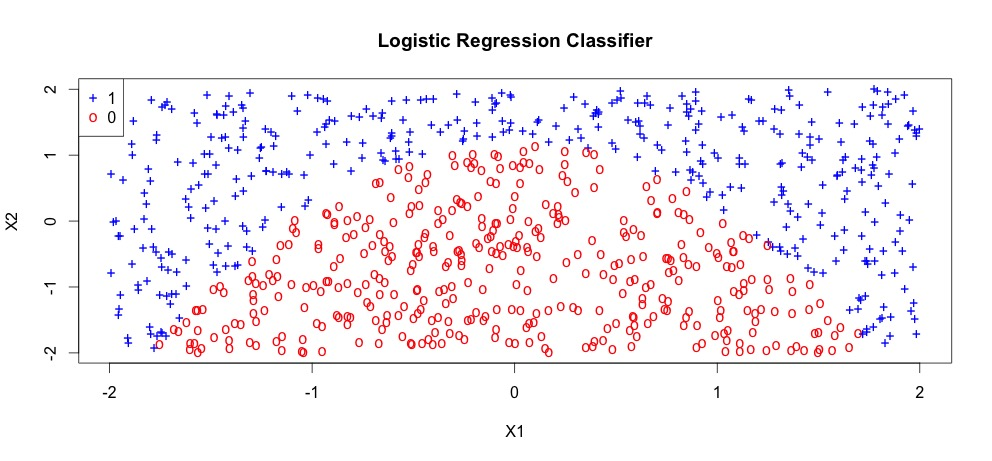
\includegraphics[scale=.4]{y1_plot.jpeg}
\end{figure}

\item Classification rule drawn on the plot, corresponds to the line 
$$x_2 = -0.063 x_1 / 1.390  - 0.127 / 1.390.$$ 
This is obtained by taking the classification rule and converting it to slope-intercept form.
\begin{lstlisting}
plot(x[,1], x[,2], col=c("red","blue")[y1+1], pch = c('o', '+')[y1+1], 
     ylab="X2", xlab="X1", main='Logistic Regression Classifier')
legend('topleft', legend=unique(y1), col=c('blue', 'red'), pch=c('+', 'o'))

logistCVSlope = -coef(logisticY1)[2] / coef(logisticY1)[3]
logisticCVInt = -coef(logisticY1)[1] / coef(logisticY1)[3]
abline(a = logisticCVInt, b = logistCVSlope, col='black', lty=1, lwd=3)
\end{lstlisting}
\begin{figure}[H] \center
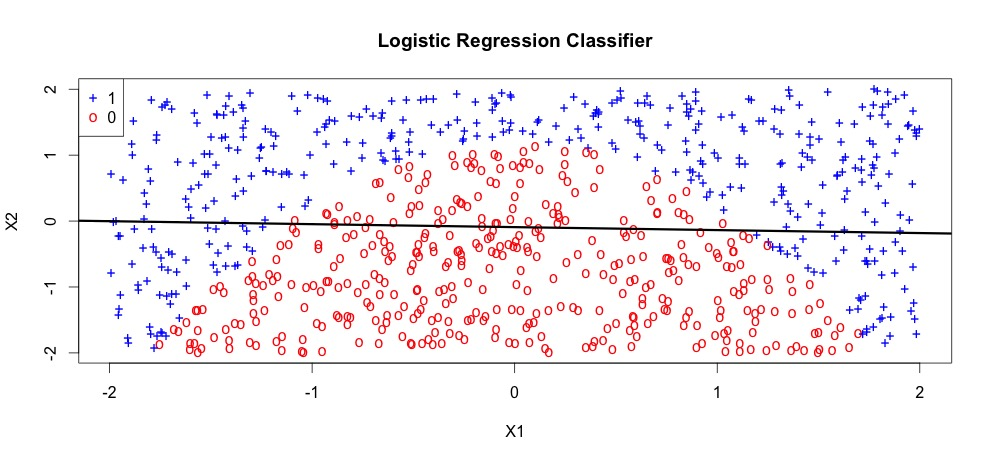
\includegraphics[scale=.4]{y1_plot2.jpeg}
\end{figure}
The classifier is clearly nonlinear (it looks like it could be quadratic or periodic with a restricted support), and yet we fit a linear rule to the data set. Not smart!
\item Similar to the plotting method described in (b), convert general form to slope-intercept form. 
\begin{lstlisting}
logisticY1.X1Square = glm(y1~x + I(x[,1]^2), family='binomial')
truePred = cbind(y1, logisticY1.X1Square$fitted.values >= 0.5)
table(Actual=truePred[,1], Predicted=truePred[,2])
\end{lstlisting}
We arrive at the conclusion that we classify to $Y=1$ if $-2322.5 -11.6 x_1 + 1955.6 x_2 + 1937.1 x_1^2 \geq 0$.
\begin{table}[H] \center
\begin{tabular}{ccc} \hline
& Predict 0 & Predict 1 \\ \hline
Actual 0 & 395 & 0 \\ 
Actual 1 & 0 & 405 \\ \hline
\end{tabular}
\end{table}
There is a perfect classification rate (0\% misclassification rate). This is definitely a better classifier, not just based on the classification rate, but it is clear that this classifier much more faithfully captures the relationship of  $y_1$ on $(x_1, x_2)$.
\item 
\begin{lstlisting}
plot(x[,1], x[,2], col=c("red","blue")[y1+1], pch = c('o', '+')[y1+1], 
     ylab="X2", xlab="X1", main='Logistic Regression Classifier')
legend('topleft', legend=unique(y1), col=c('blue', 'red'), pch=c('+', 'o'))
a = -coef(logisticY1.X1Square)[1] / coef(logisticY1.X1Square)[3]
b = -coef(logisticY1.X1Square)[2] / coef(logisticY1.X1Square)[3]
c = -coef(logisticY1.X1Square)[4] / coef(logisticY1.X1Square)[3]
curve(a + b*x + c*x^2, from=min(x[,1]), to=max(x[,1]), add = TRUE, lwd=3)
\end{lstlisting}
\begin{figure}[H] \center
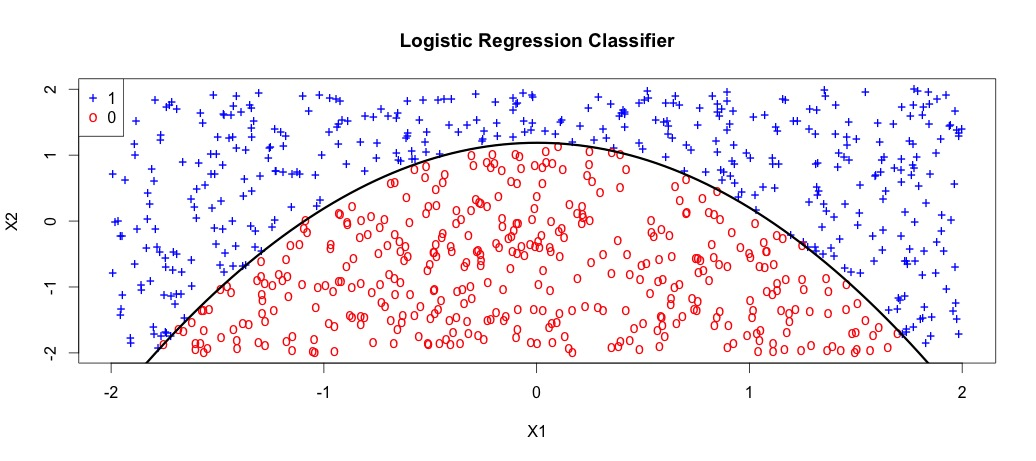
\includegraphics[scale=.4]{y1_plot3.jpeg}
\end{figure}
The classifier has a quadratic shape in $x_1$.
\item What happens when we look at $y_2$ instead of $y_1$?
\begin{lstlisting}
logisticY2 = glm(y2~x, family='binomial')
logisticY2.X1Square = glm(y2~x + I(x[,1]^2), family='binomial')
plot(x[,1], x[,2], col=c("red","blue")[y2+1], pch = c('o', '+')[y2+1], 
     ylab="X2", xlab="X1", main='Logistic Regression Classifiers with y2')
legend('topleft', legend=unique(y1), col=c('blue', 'red'), pch=c('+', 'o'))
a = -coef(logisticY2)[1] / coef(logisticY2)[3]
b = -coef(logisticY2)[2] / coef(logisticY2)[3]
abline(a = logisticCVInt, b = logistCVSlope, col='black', lty=1, lwd=3)
a = -coef(logisticY2.X1Square)[1] / coef(logisticY2.X1Square)[3]
b = -coef(logisticY2.X1Square)[2] / coef(logisticY2.X1Square)[3]
c = -coef(logisticY2.X1Square)[4] / coef(logisticY2.X1Square)[3]
curve(a + b*x + c*x^2, from=min(x[,1]), to=max(x[,1]), add = TRUE, lwd=3, col='orange')
truePredLinear = cbind(y2, logisticY2$fitted.values >= 0.5)
mean(truePredLinear[,1] != truePredLinear[,2])
truePredQuadratic = cbind(y2, logisticY2.X1Square$fitted.values >= 0.5)
mean(truePredQuadratic[,1] != truePredQuadratic[,2])
\end{lstlisting}
\begin{figure}[H] \center
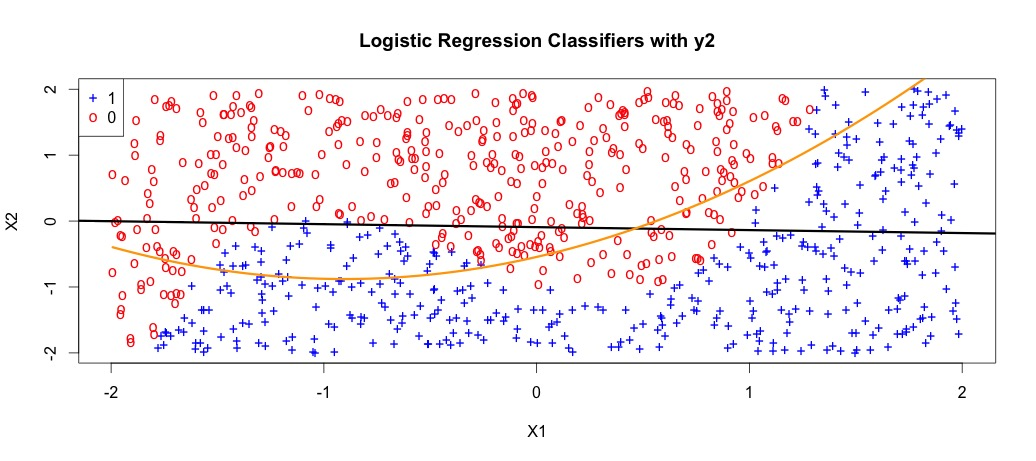
\includegraphics[scale=.4]{y2_plot1.jpeg}
\end{figure}
The linear rule has a misclassification rate of 18.5\% while the quadratic rule has a misclassification of 13.75\%. 
\item Neither rule is particularly good, because neither captures the underlying structure of the data, which appears to be higher degree than just quadratic. One approach we can do is to fit a cubic (third-order) term, which is what the relationship seems to be. If we try third-order, and classify $Y_2 = 1$ if 
$$-1455 -1541 x_1 - 1521 x_2 + 1537 x_1^2 + 1537 x_1^3 \geq 0,$$ we can achieve perfect classification.
\begin{lstlisting}
logisticY2.X1Third = glm(y2~x + I(x[,1]^2) + I(x[,1]^3), family='binomial')
plot(x[,1], x[,2], col=c("red","blue")[y2+1], pch = c('o', '+')[y2+1], 
     ylab="X2", xlab="X1", main='Logistic Regression Classifiers with y2')
legend('topleft', legend=unique(y1), col=c('blue', 'red'), pch=c('+', 'o'))
a = -coef(logisticY2.X1Third)[1] / coef(logisticY2.X1Third)[3]
b = -coef(logisticY2.X1Third)[2] / coef(logisticY2.X1Third)[3]
c = -coef(logisticY2.X1Third)[4] / coef(logisticY2.X1Third)[3]
d = -coef(logisticY2.X1Third)[5] / coef(logisticY2.X1Third)[3]
curve(a + b*x + c*x^2 + d*x^3, from=min(x[,1]), to=max(x[,1]), add = TRUE, lwd=3, col='purple')
truePredCubic = cbind(y2, logisticY2.X1Third$fitted.values >= 0.5)
mean(truePredCubic[,1] != truePredCubic[,2])
\end{lstlisting}
\begin{figure}[H] \center
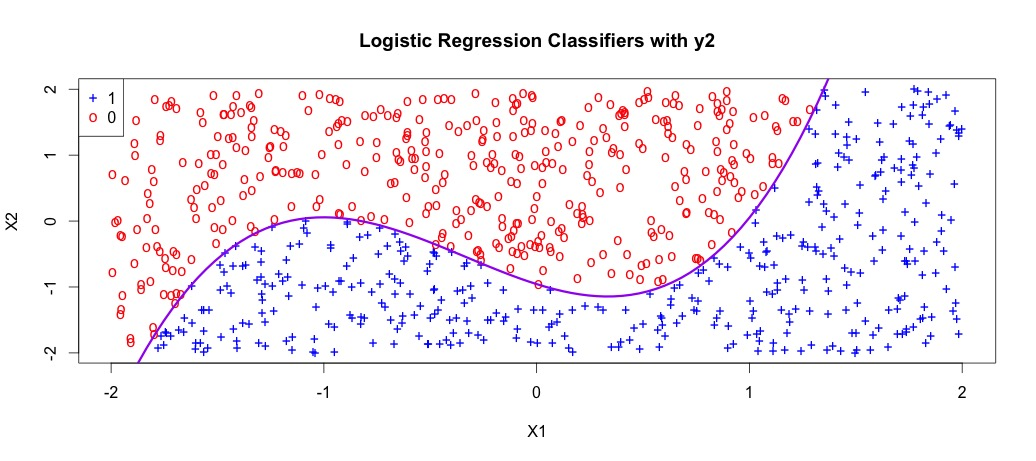
\includegraphics[scale=.4]{y2_plot2.jpeg}
\end{figure}
\item Why not keep adding more and more polynomial terms? We have seen before that we run the risk of over-fitting by adding more and more terms. That is, we begin to fine-tune a model that performs well in the sample we have, but may not generalize well to data we haven't collected yet. There are a few approaches to dealing with this over-fitting problem. We've already encountered a few in this course, as well as in previous courses. One popular way is to use cross-validation, fitting several candidate models on one set of data (the training set) and validating the model's performance on a set of data that was not used in training (the testing set), and choosing the model that performs best on the test set. Other ways would involve striking some balance between classification accuracy and the size of the model. These include AIC, BIC, Mallow's $C_p$, and many more.
\end{enumerate}
\end{document} 